\documentclass[11pt,a4paper,DIV12,pdftex]{scrartcl}
\usepackage[natbibapa]{apacite}
\usepackage[english]{babel}
\usepackage{parskip}
\usepackage{mathpazo}
\usepackage{amssymb}
\usepackage{amsmath}
\usepackage{color}
\usepackage{ifthen}
\usepackage{graphicx}
\usepackage{enumitem}
\usepackage[utf8]{inputenc}
\usepackage[dvips]{epsfig}
% Additional
\usepackage[language=bash]{listings}
\usepackage{hyperref}
\usepackage{framed}
% \usepackage[dvipsnames]{color}
\usepackage[svgnames]{xcolor}
\usepackage{soul}
% Nice colours: Gainsboro, LightGoldenrod, LightSteelBlue
% furter ref: https://www.latextemplates.com/svgnames-colors
\definecolor{shadecolor}{named}{Gainsboro}
\sethlcolor{Gainsboro}

\linespread{0.9}

\titlehead{
   
\includegraphics[height=1cm]{Universitaet_Logo_RGB.pdf} \\ \\
    Turbulent Flow Simulation on HPC-Systems \\
    Winter 2018/19 \\
    Technische Universit\"at M\"unchen 
}

\title{Worksheet 1}
% \date{\vspace*{-2cm}}
\date{\vspace*{-1cm}\today}
\author{}

\begin{document}
\maketitle
\begin{center}
	Tommaso Bianucci \\ Individual Assignment
\end{center}

\section{Physical behaviour}
\begin{shaded}
	Study the scenarios cavity, channel and channel with backward-facing step in more detail. Therefore, investigate:
\end{shaded}

\subsection{Question 1}
\begin{shaded}
	The influence of the Reynolds number on the velocity and pressure field. In particular:
\end{shaded}

\begin{enumerate}
	\item \hl{How many vortices can you observe in the cavity scenario, depending on the choice of the Reynolds number? Where are these vortices located?}

	With low Reynolds number I can observe 1 main vortex, plus 2 vortices at the bottom corners. An example of this can be seen in Fig.\ref{fig:cavity2D_50x50_Re10}, simulated with $Re = 10$.

	However as the Reynolds number increases, the main vortex moves more to the right and downwards and an additional, very irregular in shape, vortex forms on the bottom right corner. An example of this can be seen in Fig.\ref{fig:cavity2D_50x50_Re10000}, simulated with $Re = 10^4$.

	\begin{figure}[h!]
		\centering
		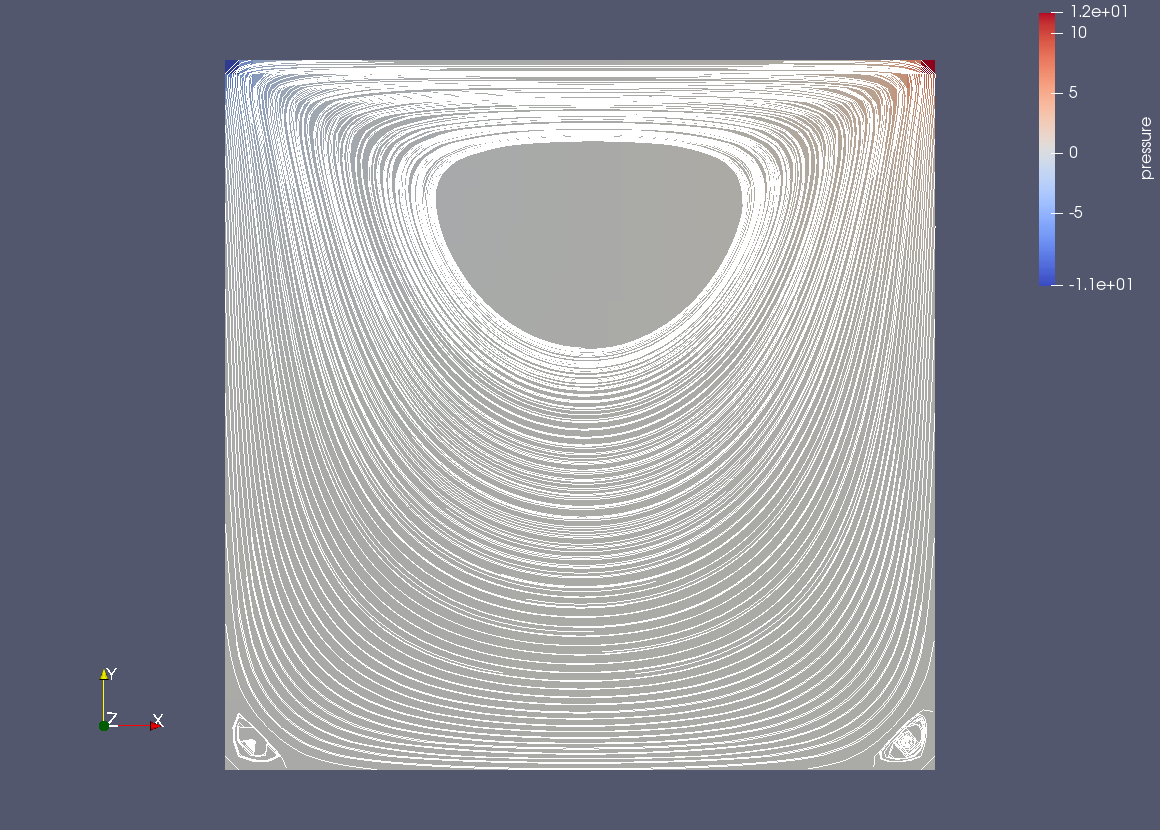
\includegraphics[width=0.7\textwidth]{Figures/cavity2D_50x50_Re10.png}
		\caption{2D cavity - 50x50 resolution - $Re = 10$} 
		\label{fig:cavity2D_50x50_Re10}
	\end{figure}

	\begin{figure}[h!]
		\centering
		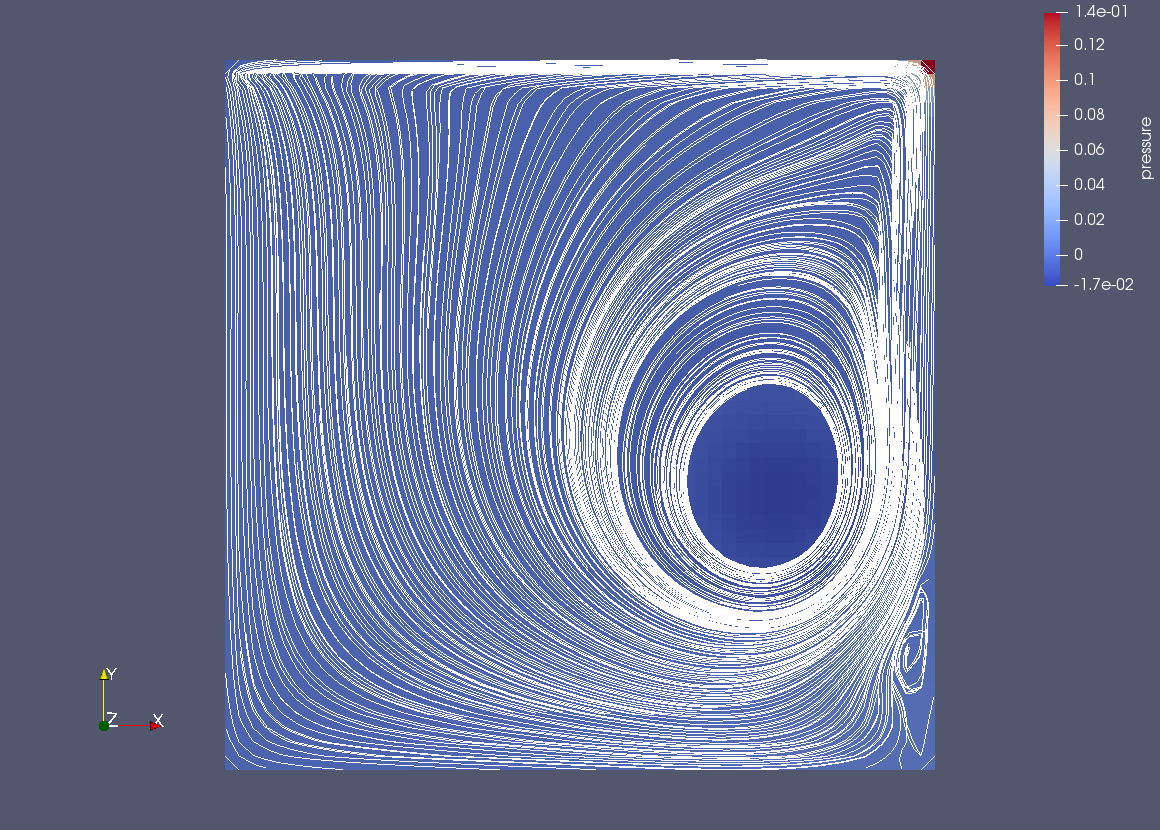
\includegraphics[width=0.7\textwidth]{Figures/cavity2D_50x50_Re10000.png}
		\caption{2D cavity - 50x50 resolution - $Re = 10^4$} 
		\label{fig:cavity2D_50x50_Re10000}
	\end{figure}

	\item \hl{How does the velocity/pressure field of the channel flow depend on the Reynolds number?}

	With low Reynolds I can observe that the distribution of the pressure field is linear and the velocity field is stronger in the center of the channel and symmetric w.r.t. its section. In this scenario, as shown in Fig.\ref{fig:Channel2D_ReComparison}.a, due to the high relevance of viscous forces, the whole fluid contained in the channel starts moving almost immediately. The pressure field almost does not change over time. The steady state is reached almost immediately.

	However with high Reynolds I can observe that the pressure field shows a sort of compression wave which moves along the channel. This is shown in Fig.\ref{fig:Channel2D_ReComparison}.b. The fluid starts moving when hit by this wave. After this transient phase, that is when the wave reaches the end of the channel, the flow stabilizes itself on the expected steady state in terms of velocity profile. However the pressure keeps oscillating for a time longer than the simulated one.

	\begin{figure}[h!]
		\begin{center}
			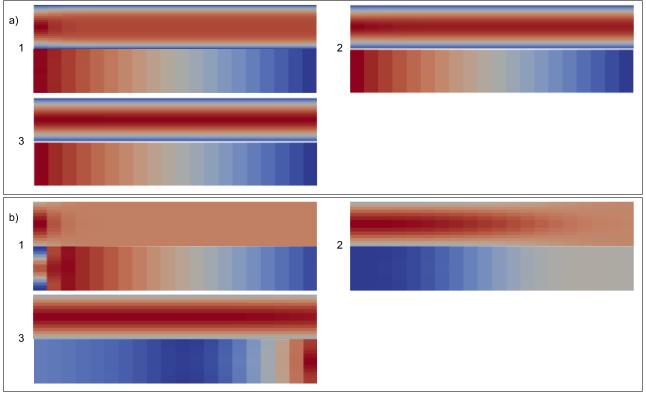
\includegraphics[width=0.9\textwidth]{Figures/Channel2D_ReComparison.png}
			\caption{Comparison of 2D channel flow behaviour with: (a) $Re=10$, (b) $Re=10^4$. For each pair of images, the upper one depicts the velocity field and the lower one the pressure field.}
			\label{fig:Channel2D_ReComparison}
		\end{center}
	\end{figure}

	\item \hl{How is the velocity/pressure field behind the backward-facing step affected by the choice of the Reynolds number?}

	With lower Reynolds number the pressure field shows a drop right behind the step\footnote{All the scenarios of this answer have a step which covers $50\%$ of the vertical domain size and $20\%$ of the horizontal one.} and a small vortex forms there, as shown in Fig.\ref{fig:Channel2D_Step_ReComparison}.a. The velocity field right behind the step has an upward vertical component, due to the vortex.

	With higher Reynolds instead, as shown in Fig.\ref{fig:Channel2D_Step_ReComparison}.b, the flow tends to form a vortex behind the step, which then migrates further downstream over time, stabilizing at a certain distance. In this scenario the flow is very slow right behind the step, since the center of the vortex is further away. Furthermore, a second vortex forms in the upper part of the channel.

	The pressure field does not show any significant change right behind the step: the low-pressure zone, corresponding to the vortex center, moves away from the step and stabilizes at a certain distance.

	Going further up in the Reynolds scale, we arrive at a point where a third small vortex forms at the bottom of the step. as shown in Fig.\ref{fig:Channel2D_Step_ReComparison}.c, the pressure right behind the step is at the same value as at the inlet. The velocity behind the step is very low and the fluid is trapped in this area.

	Furthermore the vortex in the upper part of the domain consolidates and becomes an area of more marked low pressure.

	\begin{figure}[h!]
		\begin{center}
			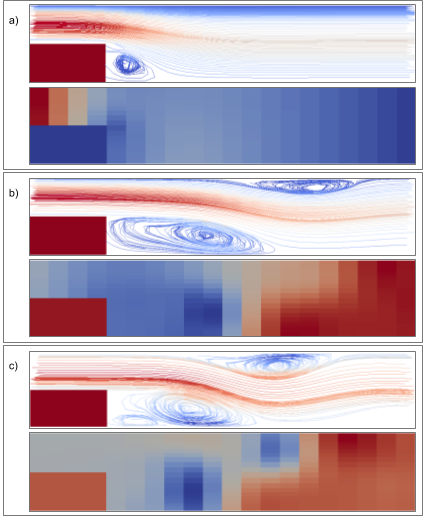
\includegraphics[width=0.75\textwidth]{Figures/Channel2D_Step_ReComparison.png}
			\caption{Comparison of 2D channel flow behaviour at steady state with: (a) $Re=50$, (b) $Re=500$, (c) $Re=10^4$. For each pair of images, the upper one depicts the velocity streamlines together with the obstacle profile and the lower one the pressure field.}
			\label{fig:Channel2D_Step_ReComparison}
		\end{center}
	\end{figure}
\end{enumerate}

\subsection{Question 2}
\begin{shaded}
	The influence of the length and height of the backward-facing step on the flow field.
\end{shaded}

Given a specific Reynolds number value, changing the height of the step determines if a vortex is formed behind it or not. I tested with a $Re=500$ and steps height of $10\%$, $50\%$ and $90\%$ of the vertical domain size. With a step heigh of $10\%$ no vortex is formed and the flow is laminar, while with steps of $50\%$ and $90\%$ a vortex forms.

For evaluating the impact of the step length, I have set a costant height of $50\%$ and tested length ratio values of $10\%$, $20\%$ and $50\%$. As expected, the length of the step does not change the physical behaviour of the flow: the three scenarios form vortices of the same size and at the same time, the only difference is that the vortex is offset to the right according to the step length.

\subsection{Question 3}
\begin{shaded}
	The influence of the used mesh on the overall accuracy and time step size. You may restrict your considerations to the channel flow scenario for this sub-task.
\end{shaded}

I tested the simple 2D channel scenario with $Re=500$, a resolution of 20x40 both with and without mesh stretching.
The timestep difference is remarkable: $2.44314\cdot10^{-4}$ with mesh stretching and $7.73515\cdot10^{-2}$ without.

This causes the run with the stretched mesh to take much longer.
But this is not the only performance change that a stretched mesh causes: profiling reveals that a relevant amount of time, $11.42\%$, is spent in calling the \verb!TanhMeshStretching::getDy()! method, which is more expensive in a stretched mesh than in a regular one\footnote{This is addressed more in depth in the next section.}.

From a qualitative perspective, the stretched mesh produces a better approximation of the effects of no-slip conditions at the top and bottom boundaries producing a slower velocity at the interface and a better approximation of the parabolic profile the solution should have. However, the general behaviour of the solution is the same regardles of the mesh used in the test.

\section{Performance}
\begin{shaded}
	Use \emph{gprof} to investigate the sequential performance of your simulation. Install \verb!gprof! on your linux system. In order to use \verb!gprof!, add the flag \verb!-pg! when compiling your program NS-EOF. After execution of a simulation, a file \verb!gmon.out! should be created in your main directory. Call \verb!gprof ./ns &> analysis.txt! to evaluate the performance statistics and write the corresponding information to a file \verb!analysis.txt!.

	What do you observe? Which routines take most of the time in your simulation? How does the VTK output affect your performance profile? How could you improve the performance of your code?
\end{shaded}

I extracted the followed statistics from a run of the 2D channel with step scenario, with a stretched mesh with resolution 20x40, $Re=500$, $vtkInterval=0.1$ and total simulation time of 10. The step used in this scenario is $50\%$ both in length and in width.

The entries in the gprof \emph{flat profile} output which display a time impact of above $10\%$ are the following:
\begin{lstlisting}
 %   cumulative   self
time  seconds    seconds  name    
14.91     16.12    16.12  MatSolve_SeqAIJ_NaturalOrdering
11.02     28.04    11.92  MatLUFactorNumeric_SeqAIJ
10.69     39.60    11.56  TanhMeshStretching::getDy(int, int) const
 9.73     50.12    10.52  MatMult_SeqAIJ
 7.77     58.53     8.41  PetscMallocValidate
\end{lstlisting}

Looking at the PETSc documentation I see that:
\begin{itemize}
	\item \verb!MatSolve_SeqAIJ_NaturalOrdering! is a solver for triangular linear systems.
	\item \verb!MatLUFactorNumeric_SeqAIJ! computes the LU matrix factorization.
	\item \verb!MatMult_SeqAIJ! computes the matrix-vector product.
\end{itemize}

While the \verb!TanhMeshStretching::getDy()! computes the extension of the given cell in the Y axis, which is used to compute interpolations or finite differences throughout the code.

Looking at the \emph{call graph} section of the gprof output, I can see that, through its children, the \verb!Simulation::plotVTK()! also causes a relevant impact on the performance:

\begin{lstlisting}

index % time    self  children  name
...
                                <spontaneous>
[5]     10.6    0.00   11.50    Simulation::plotVTK(int) [5]
                0.08   11.42    FieldIterator<FlowField>::iterate() [1]
...
\end{lstlisting}

The main cause for this high cost comes, again, for computing the Dy in the stretched mesh. Indeed if I run the simulation with exactly the same parameters, but with the \verb!stretchY="false"! parameter, the cost of \verb!Simulation::plotVTK()! halves:

\begin{lstlisting}

index % time    self  children  name
...
                                <spontaneous>
[8]      4.6    0.00    0.03    Simulation::plotVTK(int) [8]
                0.00    0.03    FieldIterator<FlowField>::iterate() [4]
...
\end{lstlisting}

The \verb!TanhMeshStretching::getDy()! is used during plotting because the velocities have to be interpolated on the staggered grid to be applied to the cell center. This is a requirement that comes from the VTK format: it is possible to specify values on cells and points, but not on edges. So a staggered grid cannot be directly represented in VTK.

A simple way to improve this performance penalty is to use a uniform mesh, if possible: in this scenario the results run with uniform and stretched meshes display the same qualitative behaviour.

Another way to retain a stretched mesh but reduce its cost, is to find another stretching scheme to use, based on a mathematical function which is cheaper to compute than \verb!tanh!.

Finally, either a lower cost approximation of \verb!tanh!, a lookup table with precomputed values or, where available, native hardware instructions could be used.

% \bibliographystyle{apacite}
% \bibliography{literature}

\end{document}

%%%%%%%%%%%
% Figure \ref{fig:placeholder} shows an example of how to include a figure.
% \begin{figure}[!ht]
% \centering
%   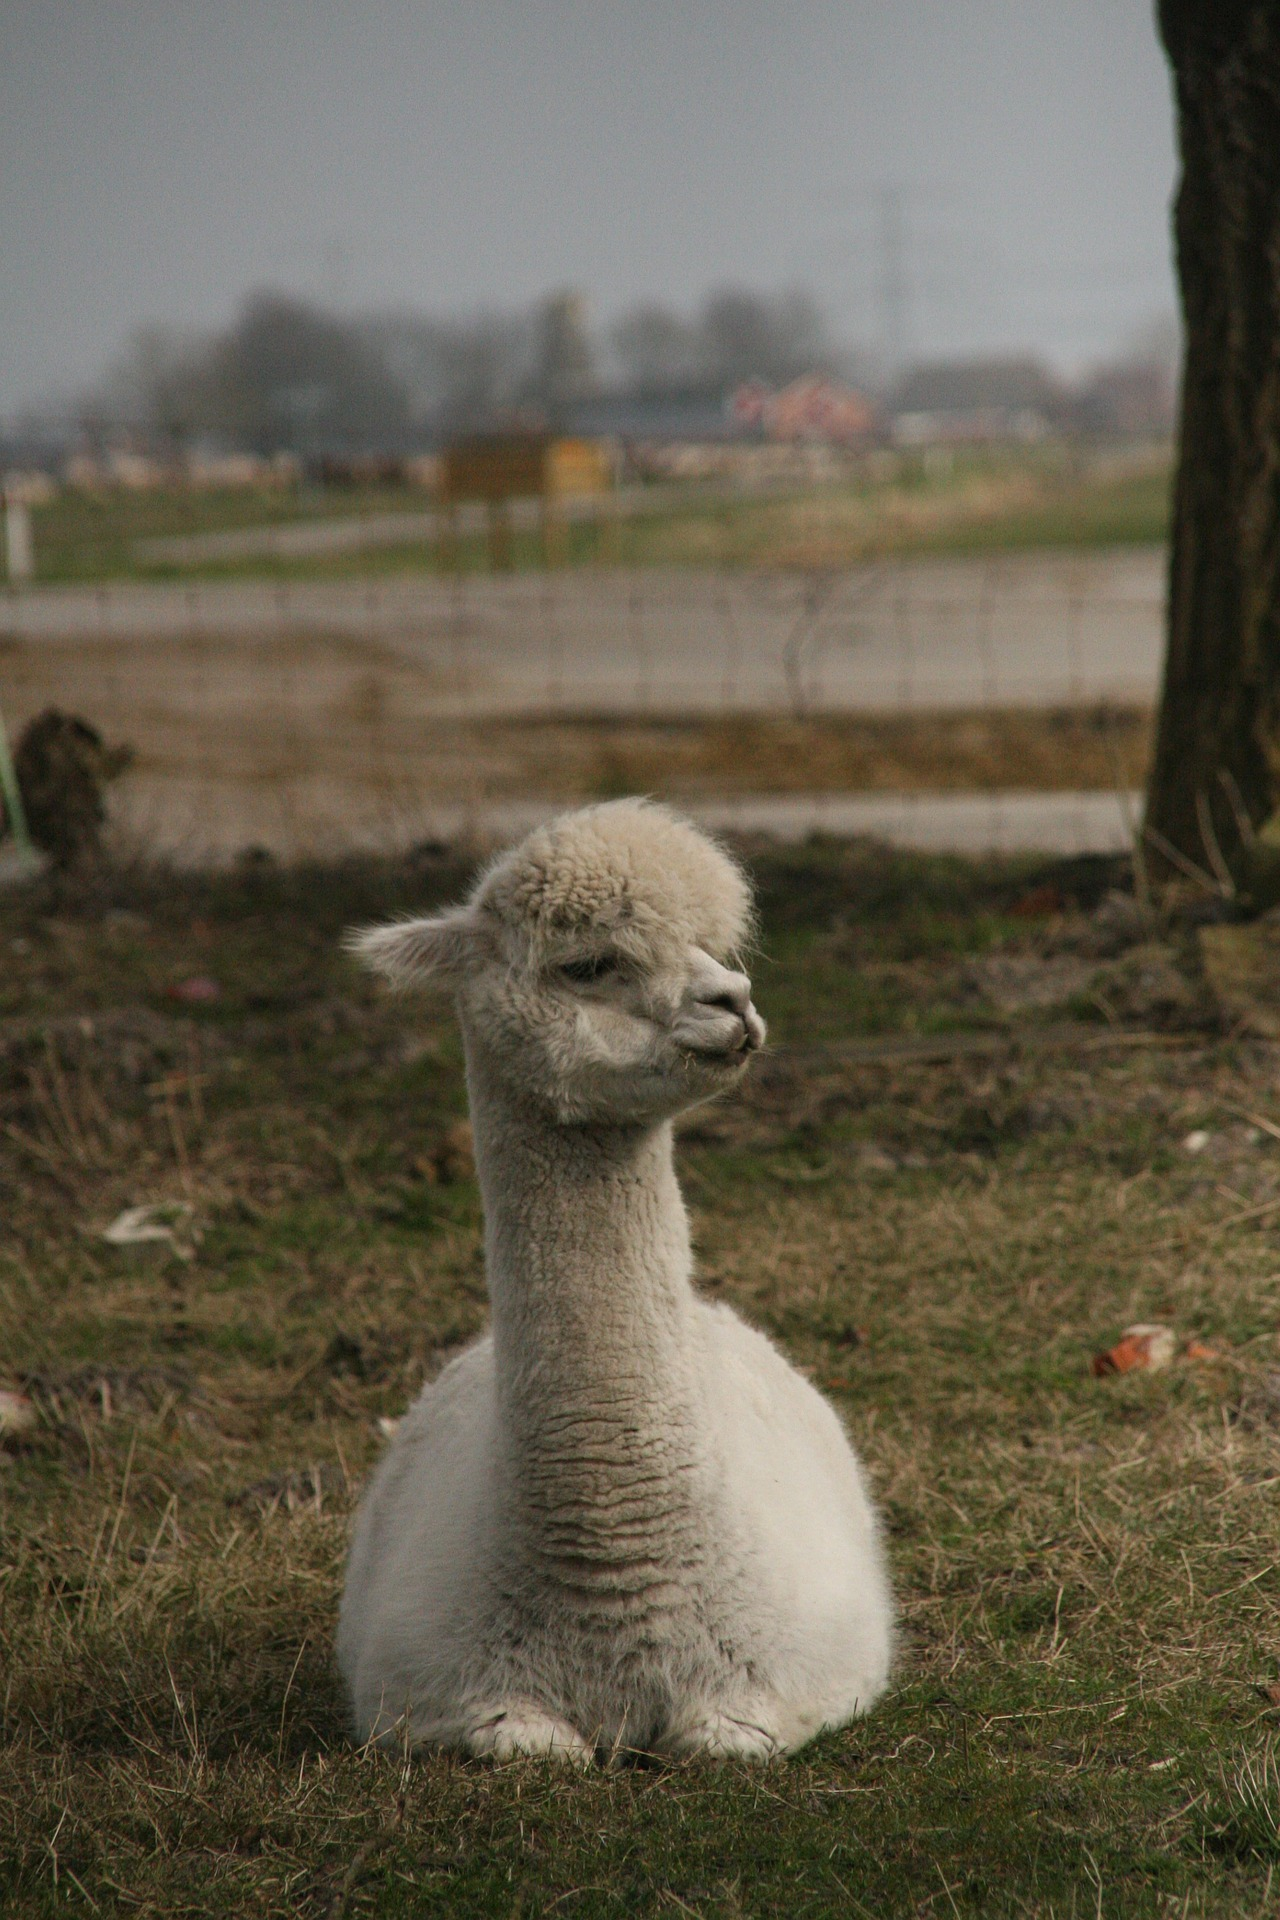
\includegraphics[width=0.3\textwidth]{Figures/placeholder.jpg}
%   \caption{Placeholder.} 
%   \label{fig:placeholder}
% \end{figure}
% \cite{jones2001taxonomy} shows an example for a citation in the next, or it can be done like this when it is not included in a sentence \citep{jones2001taxonomy}.
%%%%%%%%%%%
